\documentclass{article}
\usepackage{amsmath,amssymb,kotex,multicol, enumitem, multicol, graphicx}
\usepackage[a4paper, total={18cm, 27cm}]{geometry}

\title{예원, 수행평가 대비}
\date{\today}
\author{}
\begin{document}

\maketitle

\section{}

\begin{enumerate}[label=(\arabic*), itemsep=50pt]
    \item
    \(\begin{cases}
        y=2x\\
        x+3y=-21
    \end{cases}\)
    \item
    \(\begin{cases}
        y=-3x\\
        9x+2y=6
    \end{cases}\)
    \item
    \(\begin{cases}
        x=2y\\
        3x-2y=-4
    \end{cases}\)
    \item
    \(\begin{cases}
        y=x+2\\
        2x-3y=-8
    \end{cases}\)
    \item
    \(\begin{cases}
        y=2x-1\\
        7x-2y=14
    \end{cases}\)
    \item
    \(\begin{cases}
        x=3y+2\\
        2x+y=25
    \end{cases}\)
\end{enumerate}

\vspace*{\fill}
\noindent\textbf{답}
\begin{enumerate}[label=(\arabic*)]
    \item \(x=-3\), \(y=-6\)
    \item \(x=2\), \(y=-6\)
    \item \(x=-2\), \(y=-1\)
    \item \(x=2\), \(y=4\)
    \item \(x=4\), \(y=7\)
    \item \(x=11\), \(y=3\)
\end{enumerate}

\newpage
\section{}

\begin{enumerate}[label=(\arabic*), itemsep=50pt]
    \item
    \(\begin{cases}
        0.1x+0.2y=0.6\\
        \frac x2-\frac y3=\frac53
    \end{cases}\)
    \item
    \(\begin{cases}
        x-\frac12 y=3\\
        -0.3x+0.6y=-0.9
    \end{cases}\)
    \item
    \(\begin{cases}
        \frac 25x-\frac32y=1\\
        0.2x-0.3y=-0.4\\
    \end{cases}\)
    \item
    \(\begin{cases}
        0.2x+0.3y=3\\
        \frac 12x-\frac56y=-2
    \end{cases}\)
    \item
    \(\begin{cases}
        0.2x+0.4y=1.4\\
        \frac x3+\frac y4=\frac{13}{12}
    \end{cases}\)
    \item
    \(\begin{cases}
        0.3x+0.2y=1.1\\
        \frac{x-1}2+\frac{y+1}6=\frac13
    \end{cases}\)
\end{enumerate}

\begin{flushright}

\includegraphics[width=50pt]{jack.png}
\end{flushright}

\vspace*{\fill}
\noindent\textbf{답}
\begin{enumerate}[label=(\arabic*)]
    \item \(x=4\), \(y=1\)
    \item \(x=3\), \(y=0\)
    \item \(x=-5\), \(y=-2\)
    \item \(x=6\), \(y=6\)
    \item \(x=1\), \(y=3\)
    \item \(x=-1\), \(y=7\)
\end{enumerate}

\newpage
\section{}

\begin{enumerate}[label=(\arabic*), itemsep=50pt]
    \item
    연립방정식
    \(\begin{cases}
        x+y=6\\
        x-y=a
    \end{cases}\)
    를 만족시키는 $y$의 값이 $x$의 값의 2배일 때, 상수 $a$의 값을 구하시오.
    \item
    연립방정식
    \(\begin{cases}
        2x+y=-10\\
        -4x+y=a
    \end{cases}\)
    를 만족시키는 $y$의 값이 $x$의 값의 3배일 때, 상수 $a$의 값을 구하시오.
    \item
    연립방정식
    \(\begin{cases}
        -3x+2y=5\\
        -x+3y=2+a
    \end{cases}\)
    를 만족시키는 $y$의 값이 $x$의 값의 4배일 때, 상수 $a$의 값을 구하시오.
    \item
    연립방정식
    \(\begin{cases}
        x+2y=10\\
        3x-y=5+a
    \end{cases}\)
    를 만족시키는 $x$의 값이 $y$의 값의 3배일 때, 상수 $a$의 값을 구하시오.
    \item
    연립방정식
    \(\begin{cases}
        2x-7y=6\\
        2x+y=a
    \end{cases}\)
    를 만족시키는 $x$의 값이 $y$의 값의 5배일 때, 상수 $a$의 값을 구하시오.
    \item
    연립방정식
    \(\begin{cases}
        5x-3y=-6\\
        x+y=a
    \end{cases}\)
    를 만족시키는 $x$의 값과 $y$의 값이 서로 같을 때, 상수 $a$의 값을 구하시오.
\end{enumerate}

\vspace*{\fill}
\noindent\textbf{답}
\begin{enumerate}[label=(\arabic*)]
    \item \(-2\)
    \item \(2\)
    \item \(9\)
    \item \(11\)
    \item \(14\)
    \item \(-6\)
\end{enumerate}

\newpage
\section{}

\begin{align*}
\text{10 \% 할인된 가격} &= \text{원래 가격}\times0.9\\
\text{20 \% 할인된 가격} &= \text{원래 가격}\times0.8\\
\end{align*}

\begin{minipage}{0.5\textwidth}
\noindent (0)
\begin{itemize}
\item 1000원의 월드콘을 10\% 할인한 가격
\item 1000원의 월드콘을 20\% 할인한 가격
\item 2000원의 포카칩을 10\% 할인한 가격
\item 2000원의 포카칩을 20\% 할인한 가격
\item 650원의 라면땅을 10\% 할인한 가격
\item 650원의 라면땅을 20\% 할인한 가격
\item 1700원의 초코웨이퍼롤을 10\% 할인한 가격
\item 1700원의 초코웨이퍼롤을 20\% 할인한 가격
\end{itemize}
\vspace{80pt}
\end{minipage}
\begin{minipage}{0.4\textwidth}
    \raggedleft
    
\includegraphics[width=50pt]{onyu.png}
\end{minipage}

\begin{multicols}{2}
\begin{enumerate}[label=(\arabic*), itemsep=80pt]
    \item
    예원이는 과자와 아이스크림을 판다.
    과자의 원래 가격과 아이스크림의 원래 가격의 합은 2700원이고
    과자를 10\% 할인한 가격과 아이스크림을 20\% 할인한 가격의 합은 2310원일 때, 과자와 아이스크림의 원래 가격을 각각 구하여라.
    \item
    지현이는 가방과 모자를 판다.
    가방의 원래 가격과 모자의 원래 가격의 합은 51000원이고
    가방을 10\% 할인한 가격과 모자를 20\% 할인한 가격의 합은 44300원일 때, 가방과 모자의 원래 가격을 각각 구하여라.
    \item
    주아는 연필과 지우개를 판다.
    연필의 원래 가격과 지우개의 원래 가격의 합은 1000원이고
    연필을 10\% 할인한 가격과 지우개를 20\% 할인한 가격의 합은 860원일 때, 연필과 지우개의 원래 가격을 각각 구하여라.
    \item
    정훈이는 멜론과 매실을 판다.
    멜론의 원래 가격과 매실의 원래 가격의 합은 8600원이고
    연필을 10\% 할인한 가격과 지우개를 20\% 할인한 가격의 합은 7420원일 때, 연필과 지우개의 원래 가격을 각각 구하여라.
\end{enumerate}
\end{multicols}

\vspace*{\fill}
\noindent\textbf{답}
\begin{enumerate}[label=(\arabic*)]
    \item[(0)] 월드콘 : 900원, 800원 / 포카칩 : 1800원, 1600원 / 라면땅 : 585원, 520원 / 초코웨이퍼롤 : 1530원, 1360원
    \item 과자 : \(1500\)원, 아이스크림 : \(1200\)원
    \item 가방 : \(35000\)원, 모자 : \(16000\)원
    \item 연필 : \(600\)원, 지우개 : \(400\)원
    \item 멜론 : \(5400\)원, 매실 : \(3200\)원
\end{enumerate}


\newpage
\section{}

다음에서 $y$가 $x$에 대한 함수이면 O, 함수가 아니면 X라고 표시하고, 그 이유를 설명하여라.
\begin{multicols}{2}

\begin{enumerate}[label=(\arabic*), itemsep=30pt]
    \item
    $y$는 자연수 $x$보다 3만큼 더 큰 수
    \item
    $y$는 자연수 $x$보다 2만큼 더 작은 수
    \item
    $y$는 자연수 $x$의 네 배인 수
    \item
    $y$는 자연수 $x$보다 작은 자연수
    \item
    $y$는 자연수 $x$보다 작은 자연수의 개수
    \item
    $y$는 자연수 $x$의 약수
    \item
    $y$는 자연수 $x$의 약수의 개수
    \item
    $y$는 자연수 $x$의 배수
    \item
    $y$는 정수 $x$의 절댓값
    \item
    $y$는 고양이 $x$마리의 다리의 개수
    \item
    $y$는 닭 $x$마리의 다리의 개수
    \item
    $y$는 한 개에 2000원 포카칩의 $x$개의 가격
    \item
    $y$는 한 개에 600원 연필의 $x$개의 가격
    \item
    $y$는 원가가 $x$원인 과자를 10\% 할인한 가격
    \item
    40명의 학생들 중 여학생이 $x$명, 남학생이 $y$명
    \item
    10개의 과자들 중 $x$개를 먹었을 때 남은 과자의 수 $y$개
    \item
    시속 12km로 $x$시간동안 달린 거리 $y$ km
    \item
    20km의 거리를 시속 4km로 $x$시간동안 걸었을 때 남은 거리 $y$ km
    \item
    키가 $x$cm 인 사람의 체중 $y$ kg
    \item
    교실 안의 학생 수 $x$명과 교실 안의 온도 $y$도
    \item
    합이 5인 두 자연수 $x$와 $y$
    \item
    하루 중 낮의 길이가 $x$시간일 때 밤의 길이 $y$시간
\end{enumerate}
\end{multicols}

\vspace*{\fill}
\noindent\textbf{답}
\begin{multicols}{4}
\begin{enumerate}[label=(\arabic*)]
    \item O
    \item O
    \item O
    \item X
    \item O

    \item X
    \item O
    \item X
    \item O
    \item O

    \item O
    \item O
    \item O
    \item O
    \item O

    \item O
    \item O
    \item O
    \item X
    \item X
    \item O
    \item O
\end{enumerate}
\end{multicols}

\newpage
\section{}

\begin{enumerate}[label=(\arabic*), itemsep=80pt]
    \item
    일차함수 $y=ax-5$의 그래프가 $(4,-4)$를 지날 때, 이 그래프의 $x$절편을 구하시오. (단, $a$는 상수이다.)
    \item
    일차함수 $y=ax+3$의 그래프가 $(5,-2)$를 지날 때, 이 그래프의 $x$절편을 구하시오. (단, $a$는 상수이다.)
    \item
    일차함수 $y=ax+1$의 그래프가 $(-2,-3)$를 지날 때, 이 그래프의 $x$절편을 구하시오. (단, $a$는 상수이다.)
    \item
    일차함수 $y=2x+a$의 그래프가 $(4,14)$를 지날 때, 이 그래프의 $x$절편을 구하시오. (단, $a$는 상수이다.)
    \item
    일차함수 $y=x-a$의 그래프가 $(6,1)$를 지날 때, 이 그래프의 $x$절편을 구하시오. (단, $a$는 상수이다.)
    \item
    일차함수 $y=ax-a-2$의 그래프가 $(2,1)$를 지날 때, 이 그래프의 $x$절편을 구하시오. (단, $a$는 상수이다.)

\end{enumerate}
\vspace*{\fill}
\noindent\textbf{답}
\begin{enumerate}[label=(\arabic*)]
    \item \(20\)
    \item \(3\)
    \item \(-\frac12\)
    \item \(-3\)
    \item \(5\)
    \item \(1\)
\end{enumerate}


\newpage
\section{}

\begin{enumerate}[label=(\arabic*), itemsep=60pt]
    \item
    일차함수 $y=x-5$의 그래프를 $y$축의 방향으로 3만큼 평행이동하였을 때, 이 그래프를 그리시오, 또한 이 그래프가 지나지 않는 사분면을 구하시오.
    \item
    일차함수 $y=x+3$의 그래프를 $y$축의 방향으로 -2만큼 평행이동하였을 때, 이 그래프를 그리시오, 또한 이 그래프가 지나지 않는 사분면을 구하시오.
    \item
    일차함수 $y=2x-4$의 그래프를 $y$축의 방향으로 6만큼 평행이동하였을 때, 이 그래프를 그리시오, 또한 이 그래프가 지나지 않는 사분면을 구하시오.
    \item
    일차함수 $y=-2x-1$의 그래프를 $y$축의 방향으로 -1만큼 평행이동하였을 때, 이 그래프를 그리시오, 또한 이 그래프가 지나지 않는 사분면을 구하시오.
    \item
    일차함수 $y=-x+1$의 그래프를 $y$축의 방향으로 2만큼 평행이동하였을 때, 이 그래프를 그리시오, 또한 이 그래프가 지나지 않는 사분면을 구하시오.
    \item
    일차함수 $y=\frac12x+2$의 그래프를 $y$축의 방향으로 -4만큼 평행이동하였을 때, 이 그래프를 그리시오, 또한 이 그래프가 지나지 않는 사분면을 구하시오.
\end{enumerate}

\newpage
\noindent
\begin{minipage}{0.3\textwidth}
    \centering
    (1)
    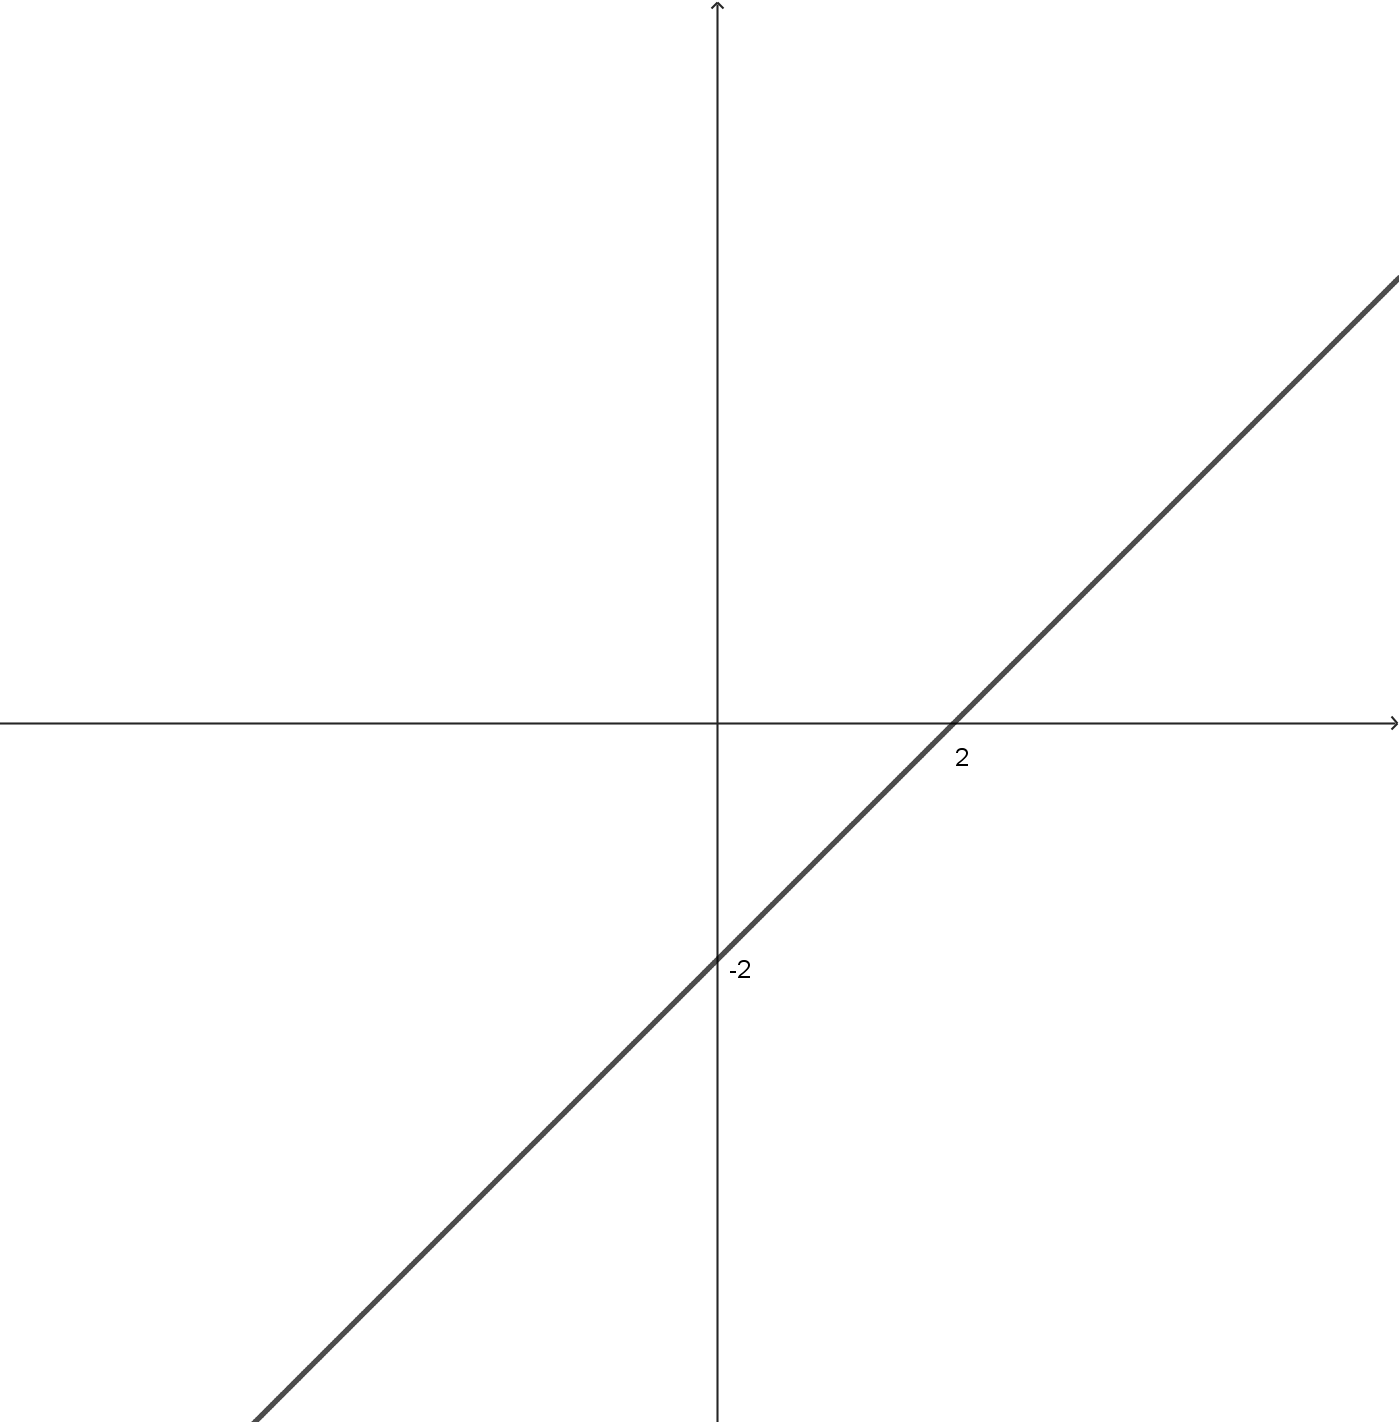
\includegraphics[width=\textwidth]{graph_1.png}\\
    $x\text{절편}=2$\\
    지나지 않는 사분면 : 제 2사분면
\end{minipage}
\begin{minipage}{0.3\textwidth}
    \centering
    (2)
    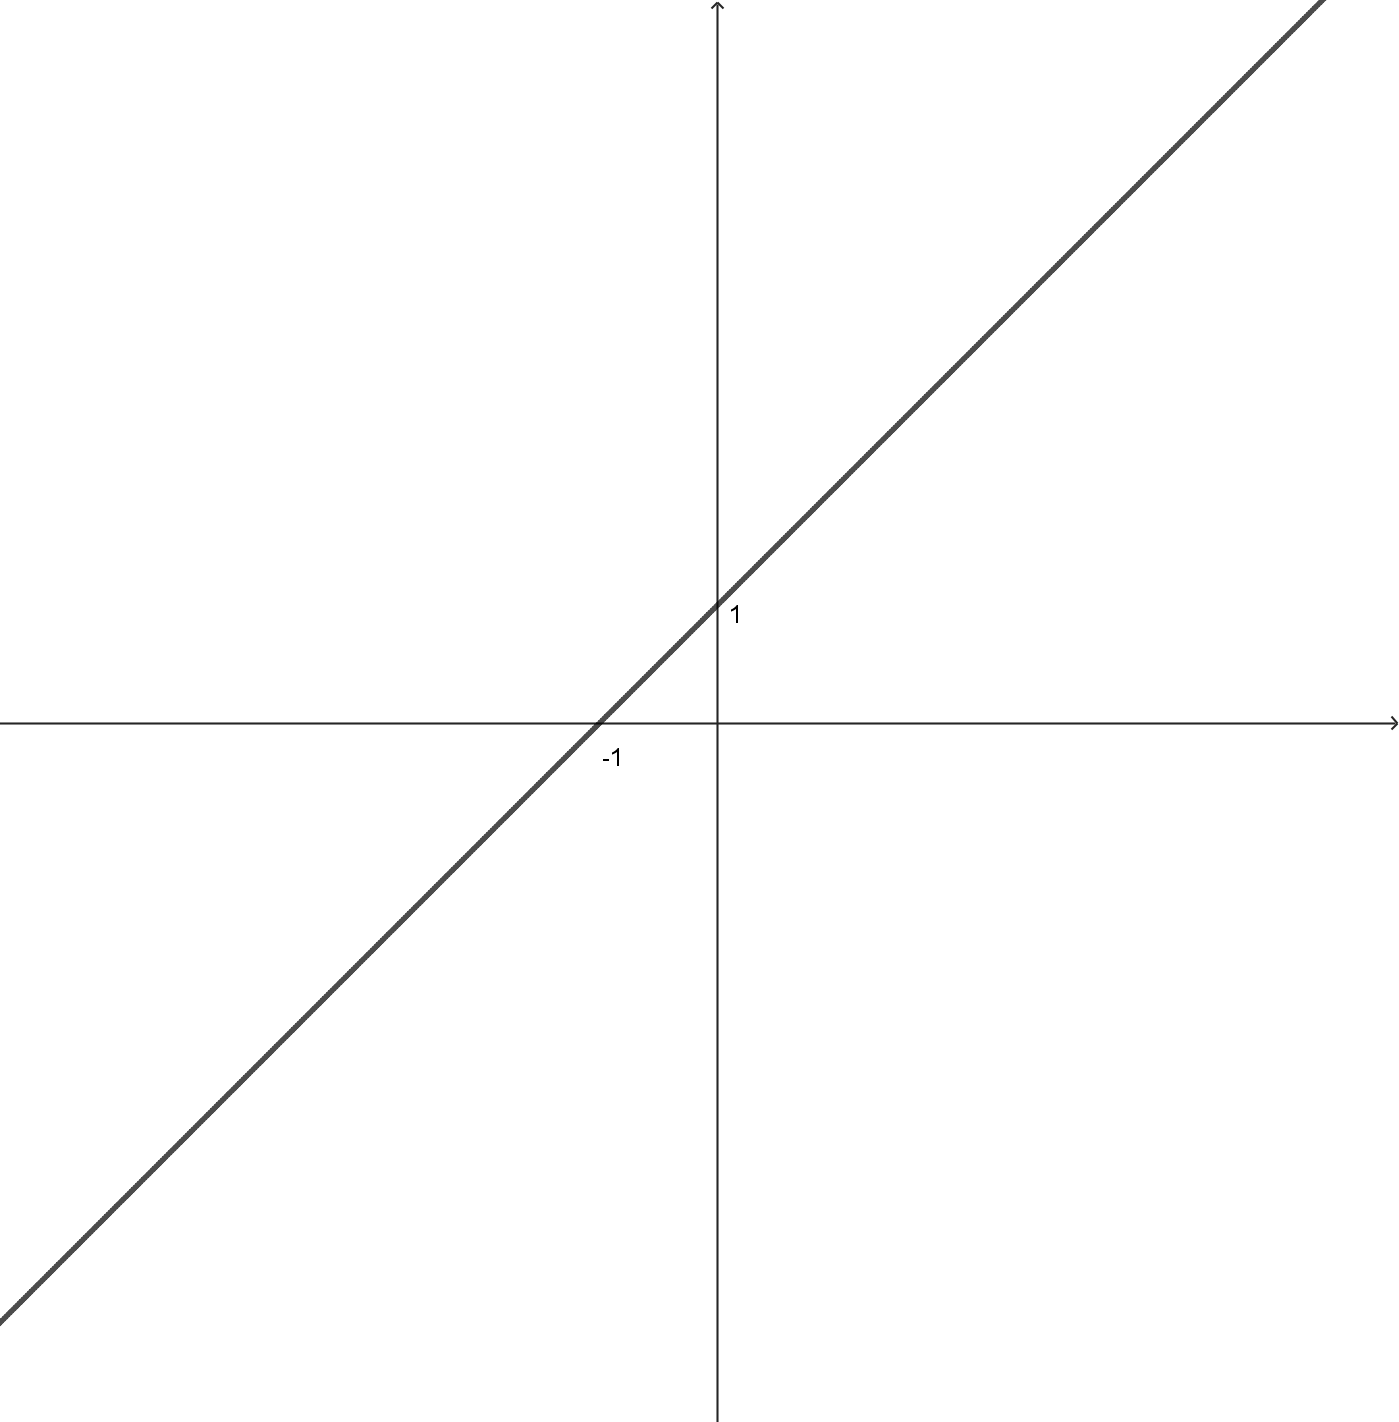
\includegraphics[width=\textwidth]{graph_2.png}\\
    $x\text{절편}=-1$\\
    지나지 않는 사분면 : 제 4사분면
\end{minipage}
\par\bigskip
\noindent
\begin{minipage}{0.3\textwidth}
    \centering
    (3)
    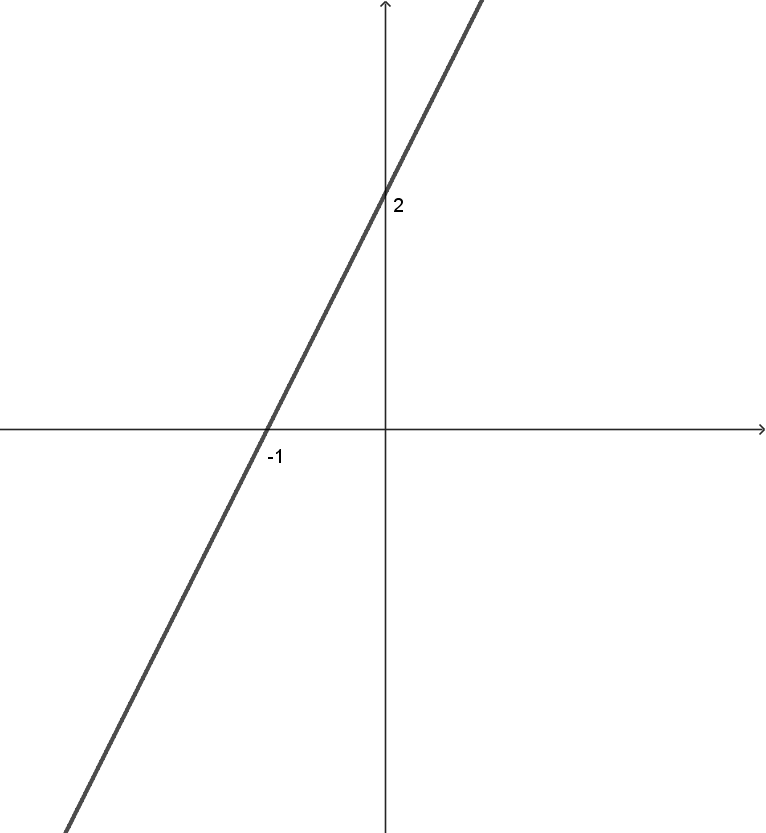
\includegraphics[width=\textwidth]{graph_3.png}\\
    $x\text{절편}=-1$\\
    지나지 않는 사분면 : 제 4사분면
\end{minipage}
\begin{minipage}{0.3\textwidth}
    \centering
    (4)
    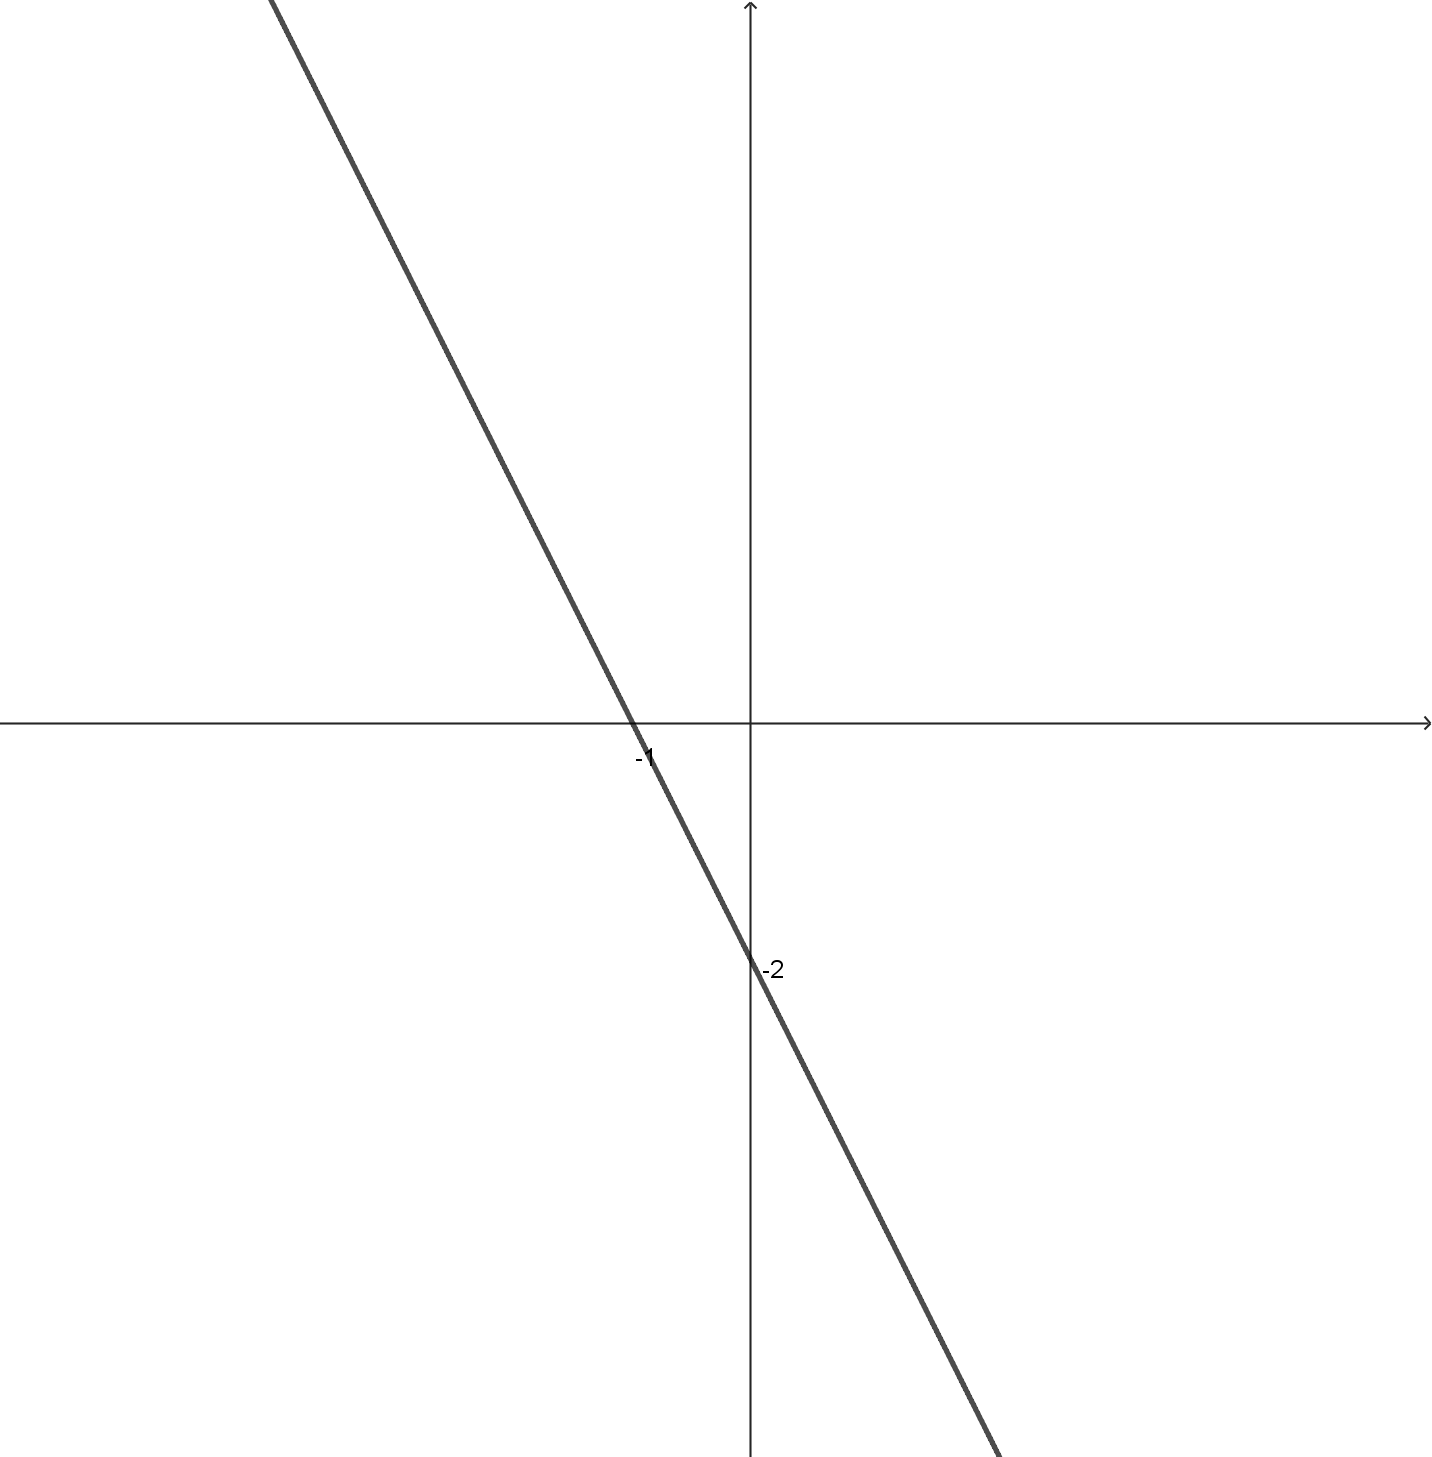
\includegraphics[width=\textwidth]{graph_4.png}\\
    $x\text{절편}=-1$\\
    지나지 않는 사분면 : 제 1사분면
\end{minipage}
\par\bigskip
\noindent
\begin{minipage}{0.3\textwidth}
    \centering
    (5)
    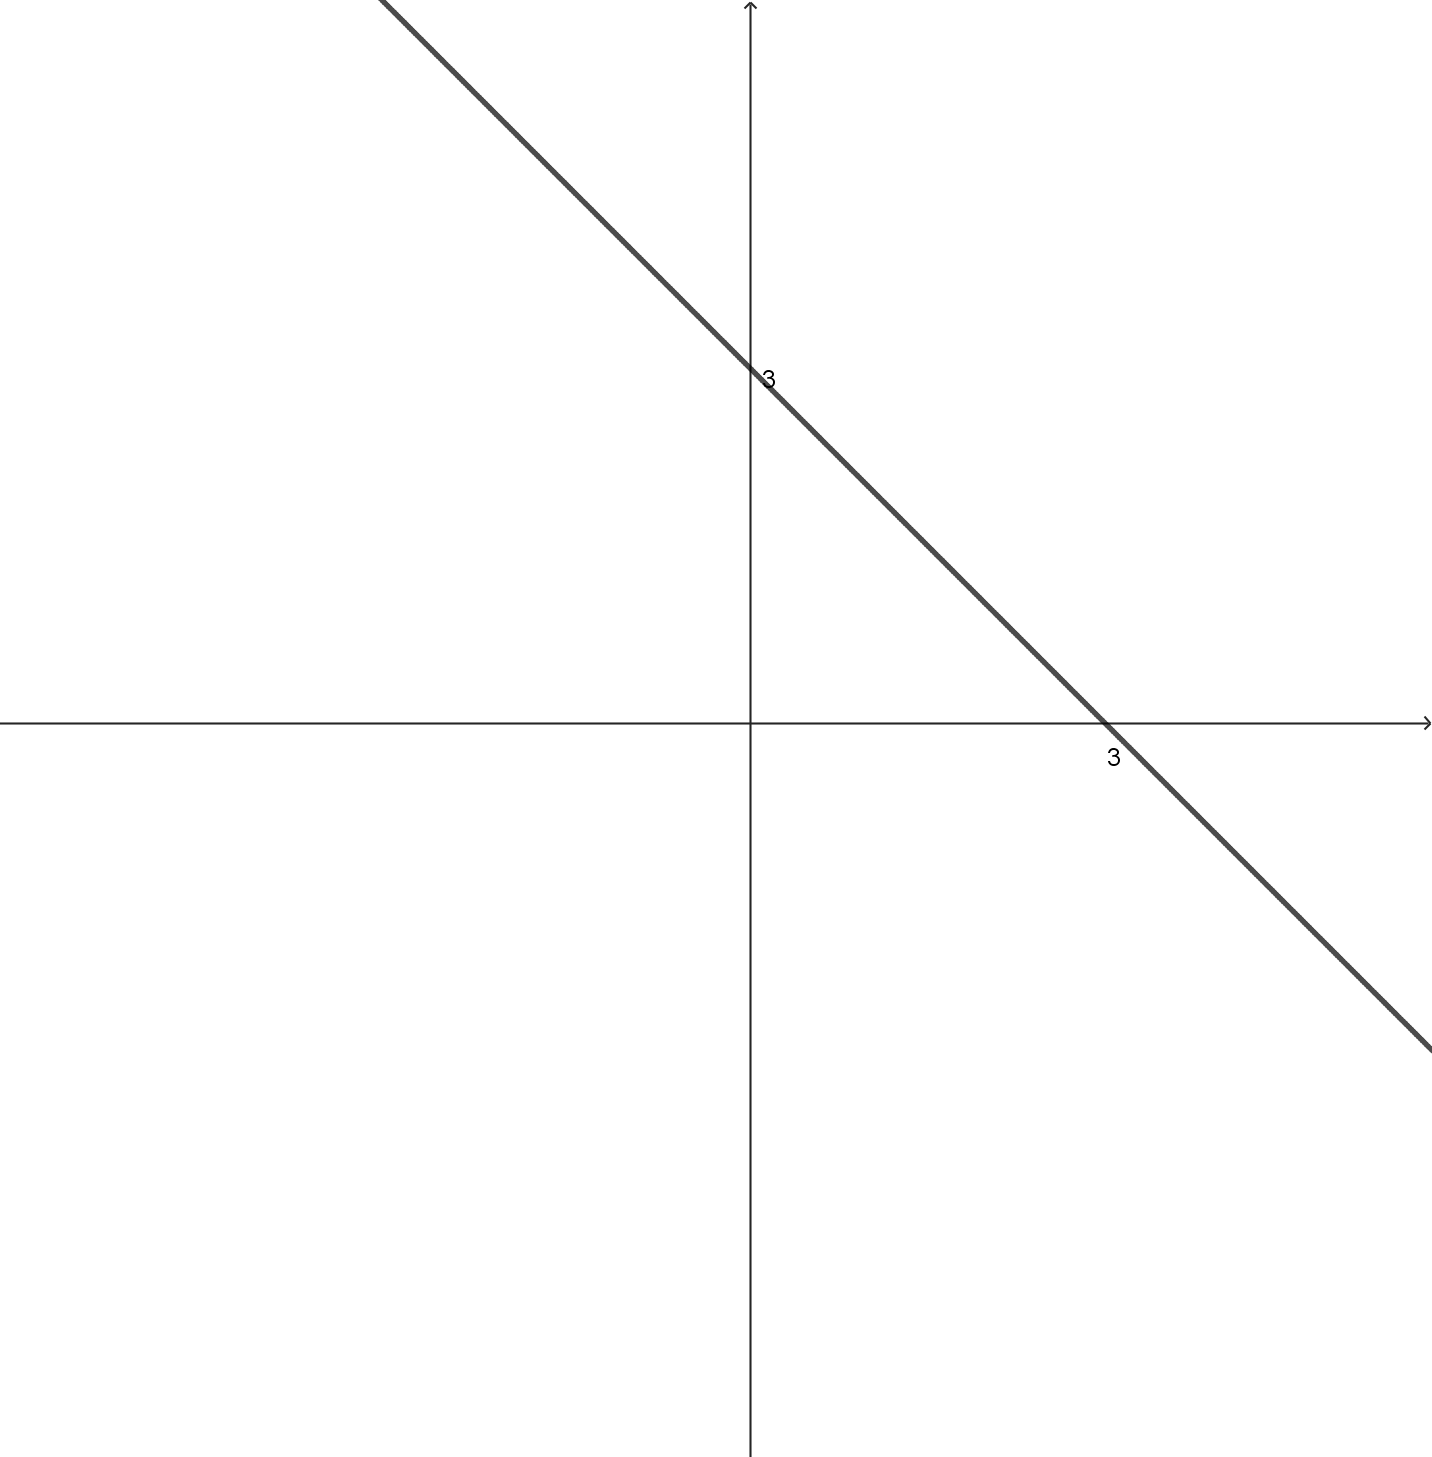
\includegraphics[width=\textwidth]{graph_5.png}\\
    $x\text{절편}=3$\\
    지나지 않는 사분면 : 제 3사분면
\end{minipage}
\begin{minipage}{0.3\textwidth}
    \centering
    (6)
    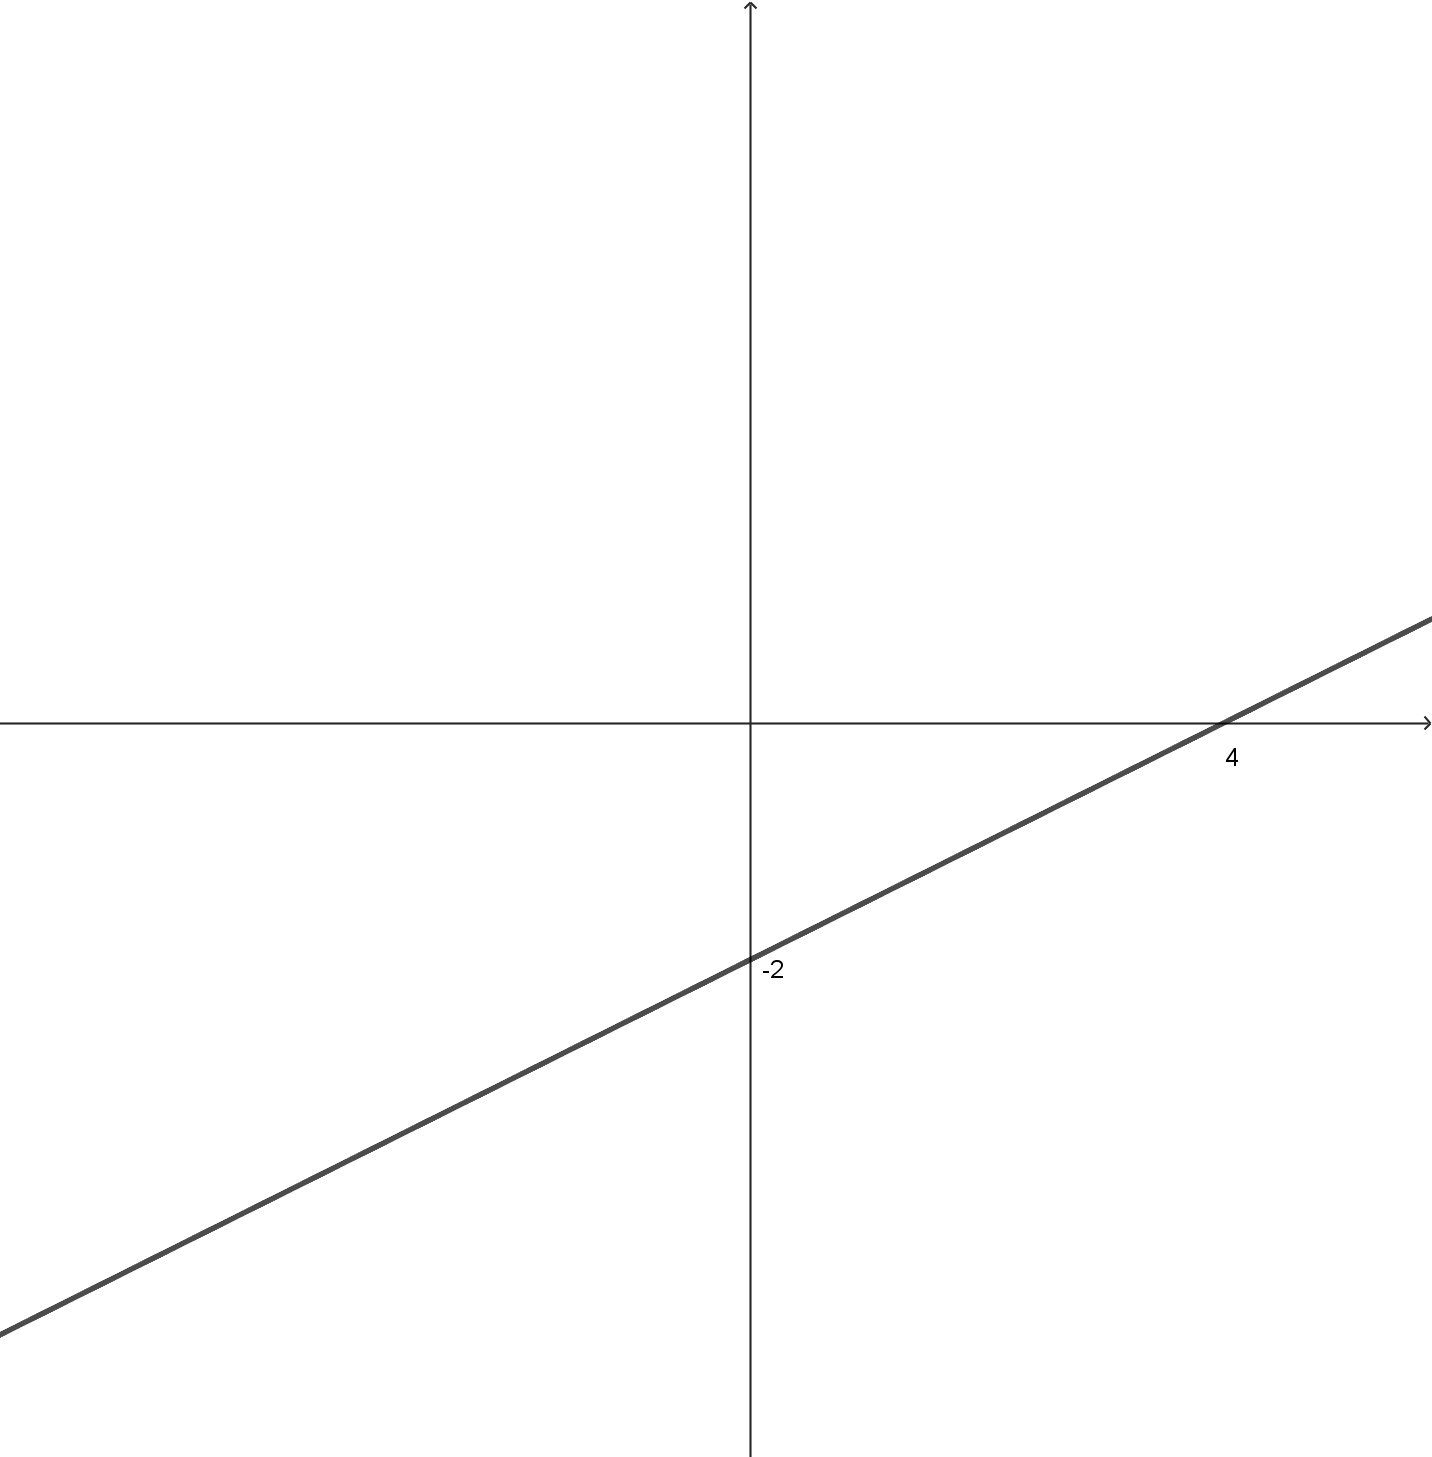
\includegraphics[width=\textwidth]{graph_6.png}\\
    $x\text{절편}=-4$\\
    지나지 않는 사분면 : 제 2사분면
\end{minipage}


\end{document}